\documentclass{article}
\usepackage[utf8]{inputenc}
\usepackage{amsmath}
\usepackage{pst-all}
\usepackage{amssymb}
\usepackage{mathrsfs}
\usepackage[french]{babel}
\usepackage{graphicx}
\usepackage{titletoc}
\usepackage{hyperref}
\usepackage{amsthm}
\usepackage{pdfpages}
\usepackage{placeins}
\usepackage{appendix}
\usepackage{MnSymbol}
\usepackage{fullpage}
\usepackage{url}
\usepackage{pgf,tikz,pgfplots}
\pgfplotsset{compat=1.15}
\usepackage{mathrsfs}
\usetikzlibrary{arrows}
\usepackage[inline]{asymptote}
\usepackage{pstricks}
\usepackage{caption}
\captionsetup{labelformat=empty}


% Environnements

\newtheorem{thm}{Théorème}[section]
\newtheorem{defn}[thm]{Définition}
\newtheorem{demo}[thm]{Démonstration}
\newtheorem{prop}[thm]{Proposition}
\newtheorem{lemme}[thm]{Lemme}
\newtheorem{rem}[thm]{Remarque}
\newtheorem{ex}[thm]{Exemple}
\newtheorem{cor}[thm]{Corollaire}
\newtheorem{corrige}[thm]{Corrigé}
\newtheorem{propr}[thm]{Propriété}
\newtheorem{conclu}[thm]{Conclusion}
\newtheorem{rappel}[thm]{Rappel}

 % Commande 
 
\newcommand{\Z}{\mathbb{Z}}
\newcommand{\N}{\mathbb{N}}
\newcommand{\R}{\mathbb{R}}
\newcommand{\C}{\mathbb{C}}
\newcommand{\F}{\mathbb{F}}
\newcommand{\Q}{\mathbb{Q}}
\newcommand{\Proj}{\mathbb{P}} % espace projectif

%Probabilités

\newcommand{\hyp}{\mathcal{H}}  %hypothèses


% Ensembles
\newcommand{\union}{\, \cup \,}     % union
\newcommand{\Union}{\, \bigcup \,}  % union (grand)
\newcommand{\inter}{\, \cap \,}     % intersection
\newcommand{\Inter}{\, \bigcap \,}  % intersection (grand)
%\newcommand{\sur}{\!\setminus\!}    % \ quotient d'ensembles


% Logique
\newcommand{\ou}{\text{ ou }}   % ou
\newcommand{\et}{\text{ et }}   % et
\newcommand{\non}{\text{non+}}    % non 
\newcommand{\avec}{\text{ avec }} %avec
\newcommand{\sinon}{\text{ sinon }} %sinon


% Parenthèses etc
\newcommand{\pars}[1]{\ensuremath{\left( #1 \right)}}               % (*) parenthèses
\newcommand{\set}[1]{\ensuremath{\left\{ #1 \right\}}}              % {*} ensemble
\newcommand{\braces}[1]{\ensuremath{\left\{ #1 \right\}}}           % {*} synonyme de \set
\newcommand{\abs}[1]{\ensuremath{\left| #1 \right|}}                % |*| valeur absolue/module
\newcommand{\norm}[1]{\ensuremath{|| \overrightarrow{#1} ||}}             % ||*|| norme vectorielle
\newcommand{\scal}[1]{\ensuremath{\left\langle #1 \right\rangle}}   % <*> produit scalaire
\newcommand{\ve}[1]{\ensuremath{\overrightarrow{#1}}}               % vecteur
\newcommand{\entiers}[1]{\ensuremath{\left[\!\left[ #1 \right]\!\right]}} % [|*|] intervalle d'entiers
\newcommand{\vect}[1]{\overrightarrow{#1}}



% Analyse
\newcommand{\eps}{\varepsilon}      % le "joli" epsilon
\newcommand{\D}{\operatorname{d}}     % d (droit)
\newcommand*{\seq}[2][0]{\ensuremath{\pars{#2}_{n \ge #1}}}     % suite (*)_{n ≥ 0}, on peut changer le 0 en argument optionnel
\newcommand*{\series}[2][0]{\ensuremath{\sum_{n \ge #1} #2}}    % série ∑_{n ≥ 0} *, on peut changer le 0 en argument optionnel
\newcommand*{\infsum}[2][0]{\ensuremath{\sum_{n \ge #1}^{\infty} #2}}   % somme infinie ∑_{n ≥ 0}^∞ *, on peut changer le 0 en argument optionnel
\newcommand{\goesto}[1][n \to \infty]{\ \underset{#1}{\longrightarrow} \ } % tend vers : --> x->0
\newcommand{\supe}[1]{\underset{#1}{\operatorname{sup}}}
\newcommand{\mini}[1]{\underset{#1}{\operatorname{min}}}
\newcommand{\infi}[1]{\underset{#1}{\operatorname{inf}}}
\newcommand{\maxi}[1]{\underset{#1}{\operatorname{max}}}
\newcommand{\norme}[2]{||#1||_{#2}}



% Trigo hyperbolique
\newcommand{\ch}{\operatorname{ch}}
\newcommand{\sh}{\operatorname{sh}}
\newcommand{\tah}{\operatorname{th}}
\newcommand{\cosinus}[1]{\operatorname{cos} \left( #1 \right)} %%%%%%%
\newcommand{\sinus}[1]{\operatorname{sin} \left( #1 \right)}

% Algèbre linéaire
\newcommand{\mat}[1]{\ensuremath{\pars{\begin{matrix} #1 \end{matrix}}}} % (**) matrice
\newcommand{\Det}{\operatorname{Det}} % Det (majuscule, \det existe déjà)
\newcommand{\diag}{\operatorname{diag}}
\newcommand{\Id}{\operatorname{Id}}


% Arithmétique
\newcommand{\legendre}[2]{\ensuremath{\left(\frac{#2}{#1}\right)}} % Symbole de Legendre
\newcommand{\Gal}{\operatorname{Gal}}


% Complexes
\newcommand{\re}{\operatorname{Re}}
\newcommand{\im}{\operatorname{Im}}


% Groupe de Lie, représentations
\newcommand{\Oronde}{\mathcal{O}}
\newcommand{\Hecke}{\mathcal{H}}
\newcommand{\Ind}{\operatorname{Ind}}
\newcommand{\GL}{\operatorname{GL}}
\newcommand{\SL}{\operatorname{SL}}
\newcommand{\Hom}{\operatorname{Hom}}
\newcommand{\End}{\operatorname{End}}
\newcommand{\Aut}{\operatorname{Aut}}
\newcommand{\Spec}{\operatorname{Spec}}
\newcommand{\Vect}{\operatorname{Vect}}
\newcommand{\Supp}{\operatorname{Supp}}
\newcommand{\ssi}{\Longleftrightarrow}  

% Déprécié
\newcommand{\GUE}{\operatorname{GUE}} % Déprécié
\newcommand{\dt}{\,.\,}

%Physique opérateur mathématiques
\newcommand{\grad}{\overrightarrow{\nabla}} %gradient avec fleche
\newcommand{\diver}[1]{\overrightarrow{\nabla}.\overrightarrow{#1}} %divergence
\newcommand{\rot}[1]{\overrightarrow{\nabla} \wedge \overrightarrow{#1}} %rotationnel
\newcommand{\df}[2]{\frac{\partial{#1}}{\partial #2}} %derivee partielle
\newcommand{\ddf}[2]{\frac{\partial^2{#1}}{\partial #2^2}} %derivee partielle seconde
\newcommand{\lap}[1]{\nabla^2 \ve{#1}} %laplacien 


%somme et produit
\newcommand{\somme}[2]{\overset{#2}{\underset{#1}{\sum}}} 
\newcommand{\produit}[2]{\overset{#2}{\underset{#1}{\Pi}}} 


%limite
\newcommand{\tendvers}[2]{\underset{#1 \rightarrow #2}{\longrightarrow}} %tend vers
\newcommand{\limite}[2]{\underset{#1 \rightarrow #2}{\operatorname{lim}}} %limite

\newcommand{\poubelle}[1]{} %fonction poubelle prend quelque chose en argument mais ne renvoie rien 

%physique
\newcommand{\cste}{\operatorname{cste}} %constante
\newcommand{\moy}[1]{\left< #1 \right>}  %valeur moyenne
\newcommand{\U}[1]{\vect{u}_{#1}}

\parindent0pt %retirer l'indentation



\date{Le 27 Mai 2020}
\begin{document}
\newpage

\title{\Huge{Rapport de projet de simulation numérique \\ \textbf{Malin comme un...blob\\}
}}
\vspace{0.5cm}


\maketitle


\begin{center}
    \rule{0.9\linewidth}{0.5pt}\\
        \vspace{5mm}
        Groupe 4\\ 
        \ \\
	    ALQUIER Rodolphe\\
      BALANNEC Ancelin\\
      CAVALIER Pierre\\
      CONTENTIN Théo\\
      HARDY Paul\\
	    \ \\
		Université Paris-Saclay\\
		L2 Double Licence Maths-Physique\\
        \vspace{5mm}	
\rule{0.9\linewidth}{0.5pt}
\vspace{0.5cm}
\end{center}

\begin{center}
\begin{minipage}{.5\textwidth}%
\psset{unit=1in,linewidth=4pt} %paramétrage des unités pour pstricks
  %\rput(10,2){
\includegraphics[width=4cm]{logo.png}}
  \centerline{
\includegraphics[width=5cm]{logo.png}}


\end{minipage}%
\hfill
\begin{minipage}{.5\textwidth}%
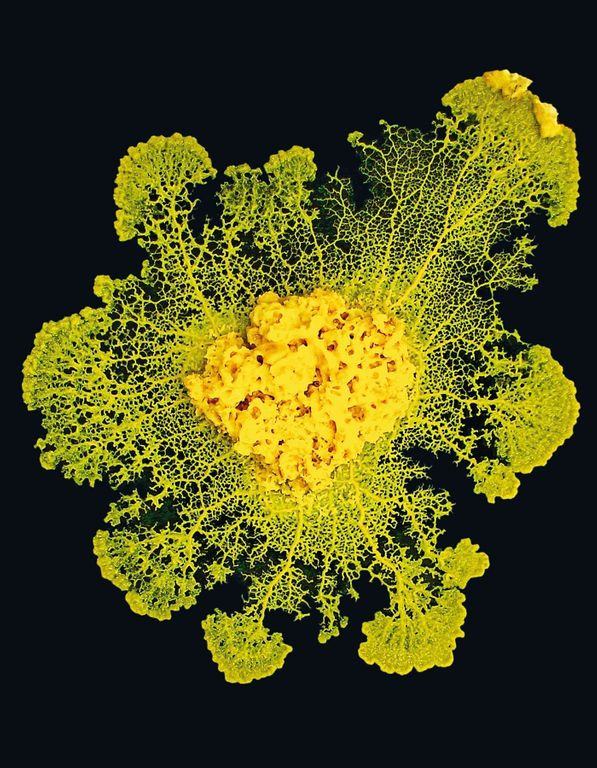
\includegraphics[width=6cm]{blob.jpg}
\end{minipage}
\end{center}


\begin{document}
\maketitle
\newpage

\tableofcontents

\newpage
\section{\Large{\texbf{Introduction}}}
\hspace*{1cm} Durant ce projet, nous avons travaillé sur "le blob"; cet organisme unicellulaire qui peut croître de plusieurs centimètres par heure et devient donc une cellule macroscopique. Le \textit{Physarum polycephalum}, de son vrai nom, peut créer des structures internes, des ramifications permettant d'acheminer la nourriture des sources aux puits. Dans ce rapport, nous avons cherché à modéliser un blob de la manière la plus simple possible : des points (ou nœuds) et des branches (ou ramifications). Nous avons fait varier plusieurs paramètres afin de balayer le plus de dispositions possibles. Pour identifier les nœuds, nous les avons numérotés de $0$ à $N-1$ avec $N$ le nombre total de points (N est un carré d'entier pour le maillage rectangulaire) de cette manière :

\begin{center}
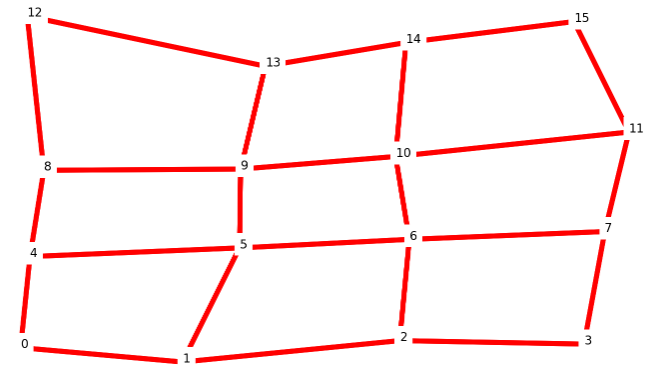
\includegraphics[width=12cm]{arrangement.png}
\end{center}

\\
\section{Présentation du modèle}
\hspace*{1cm} On  suppose  qu’à l'état initial  le  blob  est  un  réseau  de $N$ nœuds  tous  ́équivalents numérotés  de $0$ à $N-1$. Ces nœuds sont reliés entre eux par des branches dans lesquelles circuleront les nutriments. Les branches ont des longueurs et diamètres (ou épaisseurs) variables . Le débit $Q_{ij}$ dans la branche reliant le nœud $i$ au nœud $j$ est donné par la loi de Poiseuille :
\begin{center}
\begin{equation}
 Q_{ij} = \frac{\pi r^{4}}{8 \eta L_{ij}} (p_{j} - p_{i}) = \frac{D_{ij}}{L_{ij}} (p_{j} - p_{i}) 
\end{equation}
\end{center}
\ \\

où, $L_{ij}$ est la longueur de la branche, $\eta$ est la viscosité du liquide, $p_{i}$ et $p_{j}$ les pressions au niveau des nœuds $i$ et $j$. Au niveau du nœud $i$, le débit est positif lorsque le fluide va vers celui-ci. Comme la viscosité est la même partout, on introduit la conductivité ${D_{ij}$.\\
Si le nœud $k$ est une source, $\somme{j}{}Q_{kj}=I_{k} < 0$.  Ici $I_{k}$ est  le  débit  total  sortant  du  nœud. De même, si le nœud $l$ est un puits, $\somme{j}{}Q_{lj}=I_{l} >0$. Pour les autres nœuds $i$, la conservation du débit s’ecrit : $\somme{j}{}Q_{ij}=I_{i}=0$.\\
Enfin, tout ce qui rentre dans le réseau doit en ressortir. Ceci conduit à la relation : $\somme{k}{}I_{k}+\somme{l}{}I_{l}= 0$.\\
\ \\
\ \\
\ \\
\ \\
On remarque qu’il est possible de déterminer les pressions $p_{i}$ de tous les nœuds en résolvant un système de N ́équations à N inconnues, ce qui donne $AP=I$ avec $A$ une matrice ($N\times N$), $P$ un vecteur à $N$ dimensions où la i-ème ligne correspond à la pression $p_{i}$ , et $I$ est un vecteur à $N$ dimensions dont la i-ème ligne correspond au débit total $I_{i}$ au niveau du nœud $i$.\\
En résolvant ce système on obtient toutes les pressions, et ainsi on peut calculer les débits $Q_{ij}$ dans chaque branche reliant le nœud $i$ et $j$.\\
\ \\
Le rayon (ou épaisseur) $r$ de chaque branche évolue au cours du temps. Il tend à diminuer avec le temps si le débit de nutriments le traversant est faible. En revanche si un débit $Q_{ij}$  non nul s’écoule dans la branche, son rayon est non seulement stabilisé, mais il sera d’autant plus grand que le débit sera  ́élevé (jusqu’à un certain point).\\
\\
La conductivité $D_{ij}$ ́évolue avec le temps $t$ de la manière suivante :
\begin{center}
\begin{equation}
\frac{dD_{ij}}{dt}=f(Q_{ij})-\frac{D_{ij}}{\tau}
\end{equation}
\end{center}
\ \\
Avec $\tau$ le temps caractéristique de disparition d’une branche et $f$ une fonction modélisant la réponse de la branche au débit la traversant :
\begin{center}
\begin{equation}
f(Q)=\frac{|Q|^{\gamma}}{1+|Q|^{\gamma}}
\end{equation}
\end{center}
\ \\
Et pendant un temps $dt << \tau$ nous obtenons :
\begin{center}
\begin{equation}
D_{ij}(t+dt)\approx D_{ij}(t)+(f(Q_{ij})-\frac{D_{ij}}{\tau})dt
\end{equation}
\end{center}
\ \\

\section{Résolution mathématique AP = I}
\hspace*{1cm} Comme expliqué ci-dessus on cherche la matrice $A$ qui nous permettra d'obtenir $P$ la matrice correspondant aux pressions de chaque nœud.\\
\begin{equation}
\begin{pmatrix}
    a_{11} & \cdots & a_{1N} \\ 
    \\  
    \vdots & \ddots & \vdots \\ 
    \\
    a_{N1} & \cdots & a_{NN}
    \end{pmatrix}
    \times
\begin{pmatrix} p_{1} \\ 
                \\
                \vdots \\ 
                \\ 
                p_{N}
                \end{pmatrix}
    =
\begin{pmatrix} I_{1} \\ 
                \\
                \vdots \\ 
                \\  
                I_{N}
                \end{pmatrix} \end{equation}
\\

Où

\\

\begin{equation} I_{i} = \somme{\text{j}}{} Q_{ij} \end{equation}

\\
Or $Q_{ij}$ est nul si $i$ et $j$ ne sont pas voisins, on note ainsi $V[i]$ le voisinage de $I$ et ainsi :
\\
\begin{equation} I_{i} = \somme{j \in V[i]}{}\frac{D_{ij}}{L_{ij}} (p_{j} - p_{i}) \end{equation}

On obtient finalement :


\begin{equation} a_{ij} = \begin{cases}
-\somme{j \in V[i]}{}\frac{D_{ij}}{L_{ij}} \hspace*{0.433cm} \text{si} \hspace*{0.1cm} \text{$j = i$} \\
\\  %Enlever le "\\" de cette ligne pour enlever l'espace sur le pdf
\frac{D_{ij}}{L_{ij}} \hspace*{1.40cm} \text{si} \hspace*{0.1cm} \text{$j \in V[i]$} \\
\\ %Enlever le "\\" de cette ligne pour enlever l'espace sur le pdf
0 \hspace*{1.775cm} \text{si} \hspace*{0.1cm} \text{$j \not\in V[i]$}
\end{cases}\end{equation}
\\


Dans notre cas, la matrice A est de rang $N-1$ et pour résoudre ce système, on utilise la méthode des moindres carrés avec le module \textbf{np.linalg.lstsq} de Numpy.

\section{Résolution informatique}

\hspace*{1cm} Pour répondre au problème qui nous a été posé nous avons choisi de travailler avec deux classes, une pour les nœuds du réseau et une pour le blob en lui même.\\

\hspace*{1cm}La classe des noeuds nous permet de répertorier toutes les informations sur un nœud. À un point $n$ on associe ses coordonnés $x$ et $y$ comme vu précedemment et une légère fluctuation aléatoire dans un carré de côté 0.5 et de centre le point. À ce point, on associe sa liste de voisins (create$\_$voisins) et à partir de cette dernière on obtient la distance par rapport aux voisins (get$\_$L) et la conductivité (get$\_$D) par rapport à ses voisins.\\

\hspace*{1cm}À partir de cette classe, nous avons créer la classe blob qui génère tout le maillage avec des options qui permettent différents type de situations ainsi qu'une répartition des puits et des sources aussi bien constante que variable. De plus cette classe initialise aussi les paramètres des nœuds ainsi que l'intensité des sources et des puits.\\

\hspace*{1cm}De plus, nous avons rajouté une fonction pour répresenter graphiquement chaque partie du blob (plot (plot3D dans le cas à trois dimensions)), que ce soit les nœuds (plot$\_$noeud), les branches (plot$\_$branch), les puits (plot$\_$puits), les sources (plot$\_$sources). Nous avons ajouté une fonction (get$\_$noeud) qui renvoie l'objet nœud correspondant à l'indice $n$ donné, ainsi que des fonctions qui calculent la matrice $A$ comme vu précedemment dans la partie 3, qui permettent d'obtenir l'intensité (get$\_$I) en un nœud et qui calculent la pression (calcule$\_$p) en un nœud donné.\\

\hspace*{1cm}Ensuite nous avons la fonction (calcule$\_$D) qui permet d'avancer à l'instant $t + dt$, à partir des données à l'instant $t$ en calculant la conductivité à partir de l'équation (4). Pour cette fonction nous avons dû résoudre une équation différentielle(equa$\_$diff).
\\
\\
\hspace*{1cm}Nous avons, en outre, créé des sous-classes de la classe noeud dont le maillage est différent (hexnoeud, Delaunoeud...) pour que ces sous-classes héritent des attributs de nœud tout en ayant la possibilité de recoder la fonction create$\_$voisins qui ne marche plus quand on sort du maillage rectangulaire.

\newpage
\section{Observations et analyse des résultats}
\hspace*{1cm}Nous avons donc testé notre blob dans la forme la plus simple, avec un puit et une source fixés. Avec $\tau$ = 1 et $\gamma$ = 1.8 et un pas de temps $dt = 0.01$ nous avons lancé la simulation ce qui donne l'évolution ci-dessous :

\begin{center}
\begin{figure}[h]
    \begin{minipage}[c]{.30\linewidth}
        \centering
        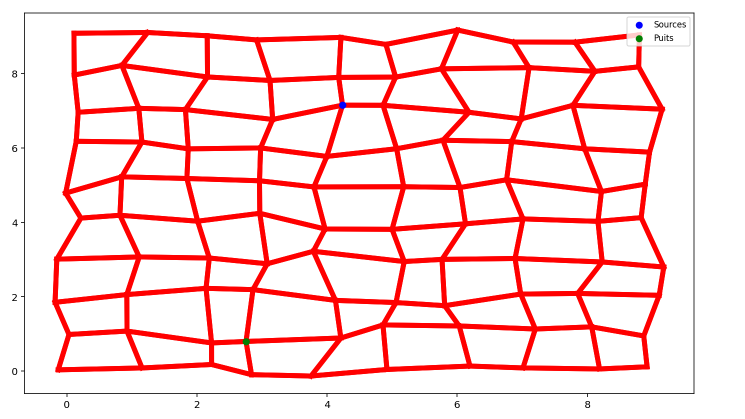
\includegraphics[width=5cm]{blob_classique_1.png}
        \caption{Situation initiale}
    \end{minipage}
    \hfill%
    \begin{minipage}[c]{.30\linewidth}
        \centering
        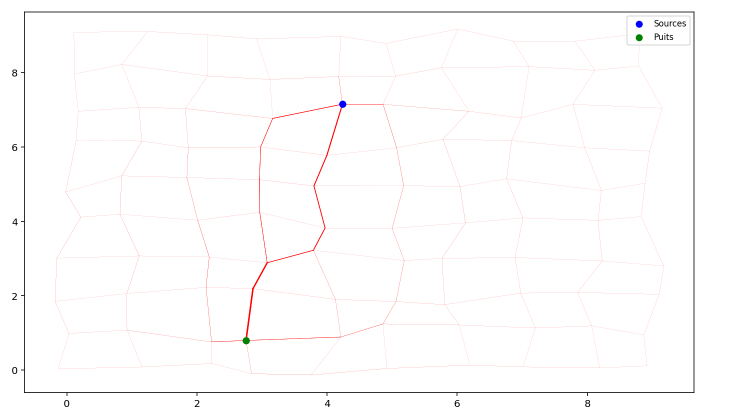
\includegraphics[width=5cm]{blob_classique_2.png}
        \caption{Après 500 itérations}
    \end{minipage}
    \hfill%
    \begin{minipage}[c]{.30\linewidth}
        \centering
        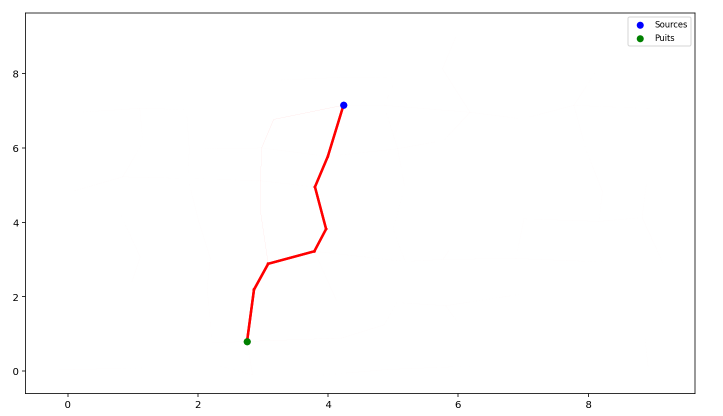
\includegraphics[width=5cm]{blob_classique_3.png}
        \caption{Après 1000 itérations}
    \end{minipage}
\end{figure}
\end{center}

%\begin{center}
%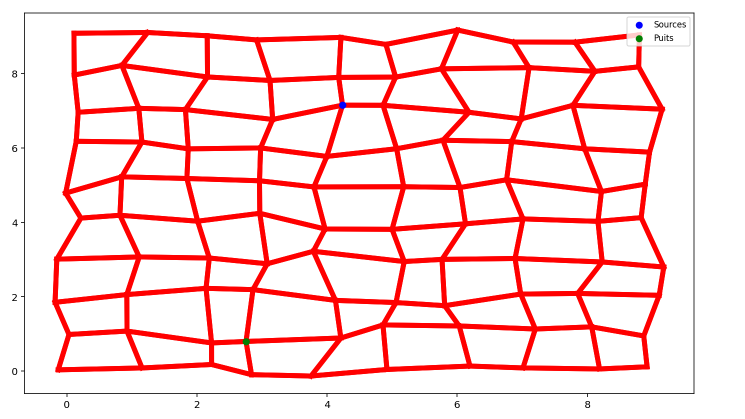
\includegraphics[width=5cm]{blob_classique_1.png} 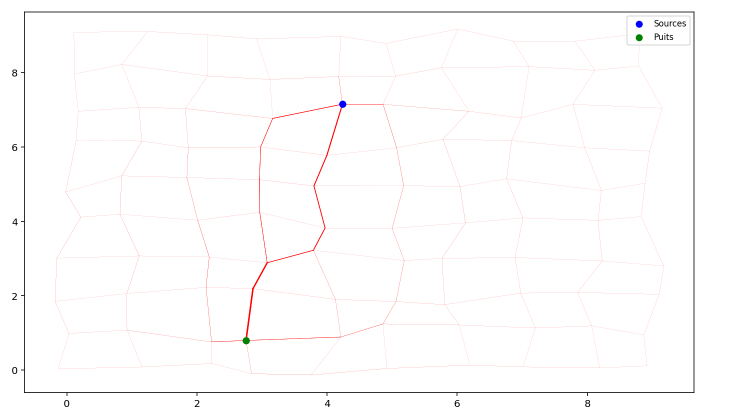
\includegraphics[width=5cm]{blob_classique_2.png} 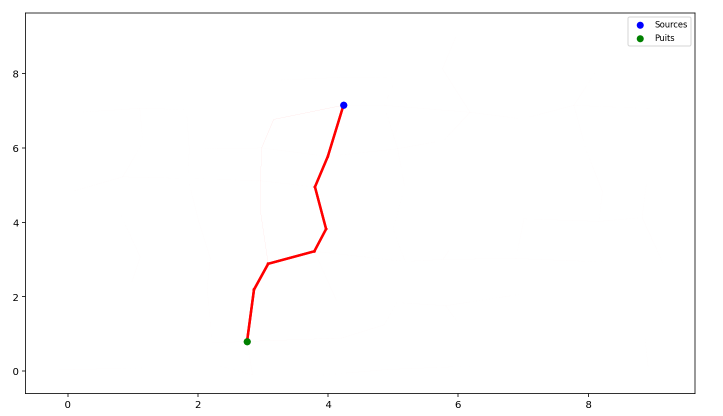
\includegraphics[width=5cm]{blob_classique_3.png}
%\hspace*{0.4cm} Situation initiale \hspace*{2cm}  Après 500 itérations \hspace*{1.8cm} Après 1000 itérations
%\end{center}

\hspace*{1cm}La simulation est donc cohérente avec la théorie, le blob crée un chemin optimisé entre le puit et la source, la dernière branche restante correspond au plus petit chemin reliant la source au puit.
\\
\hspace*{1cm}Rajoutons plusieurs puits et sources à différents endroits (toujours fixes dans le temps) et analysons les résultats après 1000 itérations. Les trois images résultantes sont donc issues de situations initiales distinctes.
\\
\begin{center}
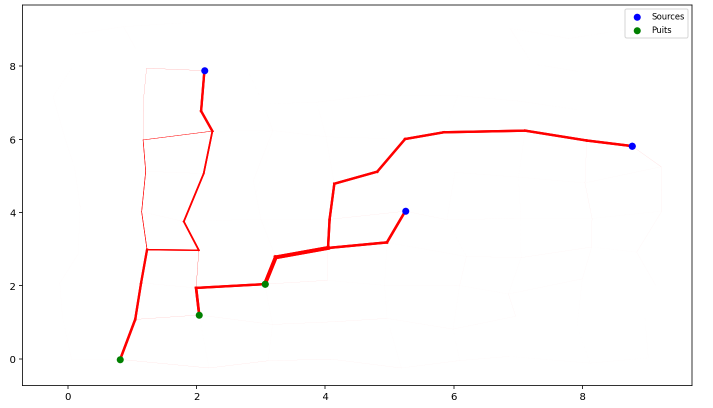
\includegraphics[width=5cm]{blob_331.png} 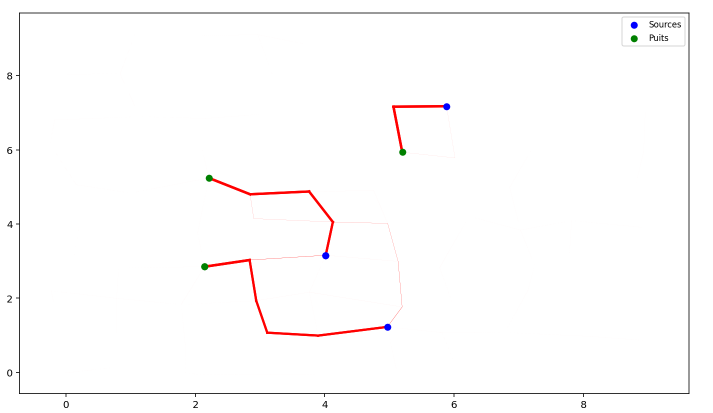
\includegraphics[width=5cm]{blob_332.png} 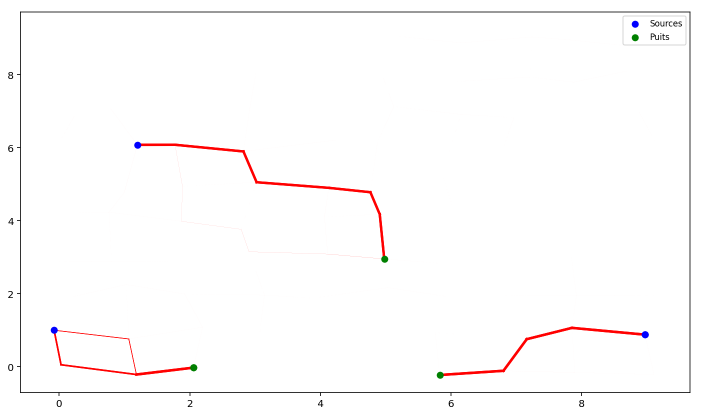
\includegraphics[width=5cm]{blob_333.png}
\end{center}
\\
\hspace*{1cm}On remarque sur ces trois exemples que la connexion entre les puits et les sources est optimale, il n'y a pas de manière plus courte de relier les sources aux puits que celle effectuée par le blob.\\
\hspace*{1cm} Nous allons désormais nous intéresser à l'impact de $\tau$ et de $\gamma$ sur l'évolution du blob. Nous avons fait varier la valeur de $\tau$ entre $0.1$ et $100$. Voici ce que nous avons observé :


\begin{center}
\begin{figure}[h]
    \begin{minipage}[c]{.30\linewidth}
        \centering
        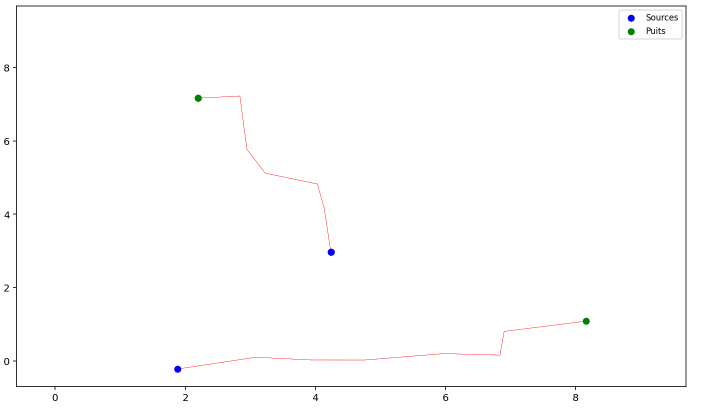
\includegraphics[width=5cm]{blob_tau1.png}
        \caption{$\tau = 0.1$}
    \end{minipage}
    \hfill%
    \begin{minipage}[c]{.30\linewidth}
        \centering
        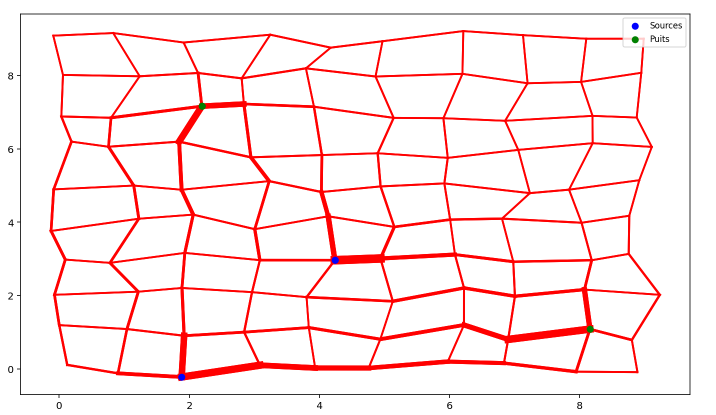
\includegraphics[width=5cm]{blob_tau2.png}
        \caption{$\tau = 10$}
    \end{minipage}
    \hfill%
    \begin{minipage}[c]{.30\linewidth}
        \centering
        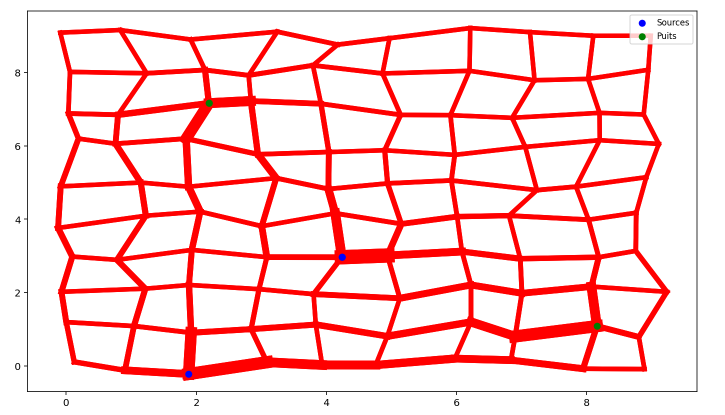
\includegraphics[width=5cm]{blob_tau3.png}
        \caption{$\tau = 100$}
    \end{minipage}
\end{figure}
\end{center}

\hspace*{1cm}Les graphes représentent respectivement l'évolution du blob à $\tau = 0.1$, $10$ et $100$ après $1000$ itérations.
On observe que plus la valeur de $\tau$ est petite, plus l'état final (l'état dans lequel il ne reste que les chemins optimisés entre les sources et les puits) est atteint rapidement. Ce résultat était prévisible puisque la dérivée temporelle de la conductivité dépend de $-\frac{1}{\tau}$. Nous voyons également que les branches au niveau des puits et des sources sont plus épaisses quand $\tau$ augmente.\\
\\
\hspace*{1cm}Nous avons étudié l'influence de $\gamma$ sur l'évolution du blob. Voici nos résultats :


\begin{figure}[h]
    \begin{minipage}[c]{.30\linewidth}
        \centering
        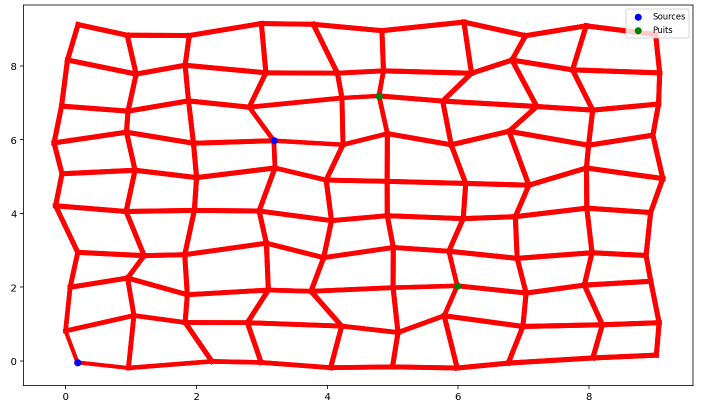
\includegraphics[width=5cm]{blob_gamma1}
        \caption{$\gamma = -1.8$}
    \end{minipage}
    \hfill%
    \begin{minipage}[c]{.30\linewidth}
        \centering
        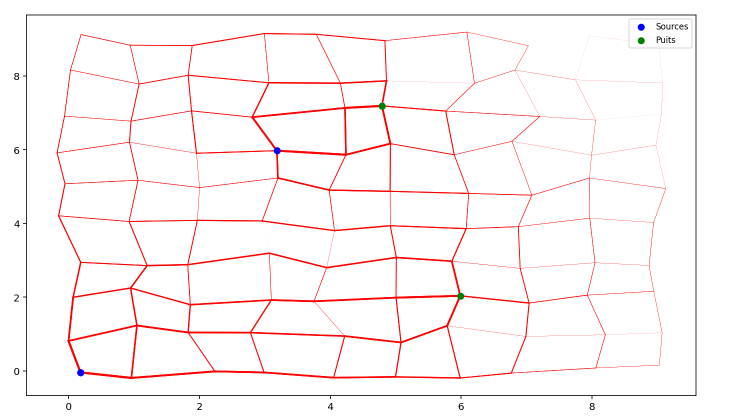
\includegraphics[width=5cm]{blob_gamma2}
        \caption{$\gamma = 0.5$}
    \end{minipage}
    \hfill%
    \begin{minipage}[c]{.30\linewidth}
        \centering
        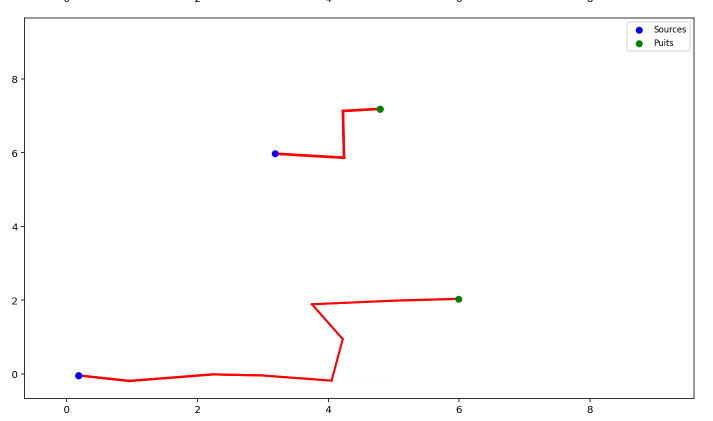
\includegraphics[width=5cm]{blob_gamma3}
        \caption{$\gamma = 5$}
    \end{minipage}
\end{figure} \\

Comme précédemment pour $\tau$ nous avons étudié la forme finale du blob après $1000$ itérations pour $\gamma = -1.8$, $0.5$ et $5$. On note que la vitesse de croissance augmente lorsque $\gamma$ augmente ce qui est logique étant donné que plus $\gamma$ est élevé plus $f(Q)$ le sera aussi et la dérivée temporelle de la conductivité dépend de $f(Q)$.
\\
\\
\hspace*{1cm}On cherche maintenant ce qu'il se passe lorsque l'on impose un débit au réseau.
\begin{figure}[h]
    \begin{minipage}[c]{.30\linewidth}
        \centering
        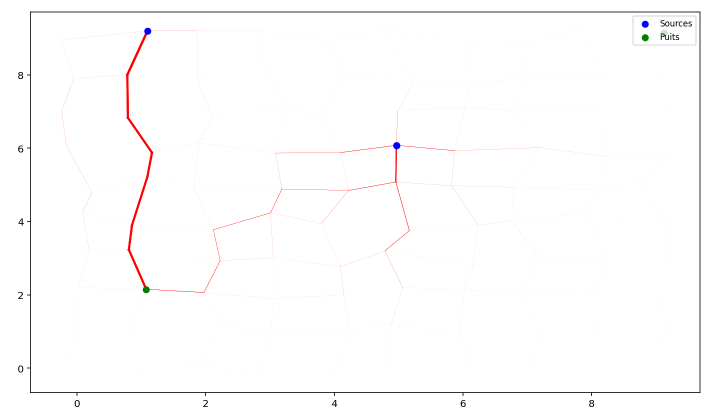
\includegraphics[width=5cm]{blob_debitvar_1.png}
        \caption{$I_{source} = -1 $ et $I_{puit} = 1 $}
    \end{minipage}
    \hfill%
    \begin{minipage}[c]{.30\linewidth}
        \centering
        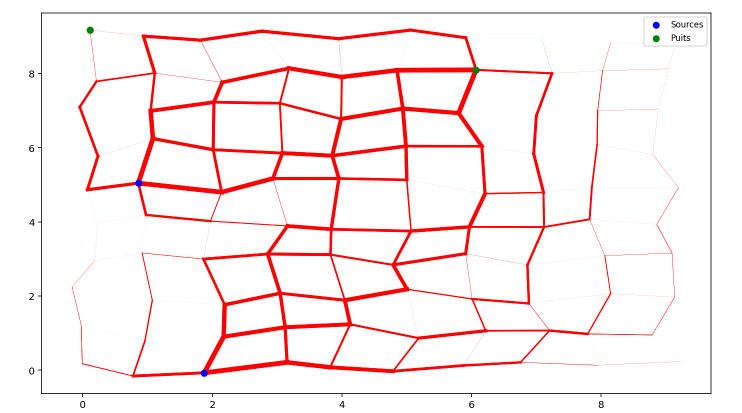
\includegraphics[width=5cm]{blob_debitvar_10.png}
        \caption{$I_{source} = -10 $ et $I_{puit} = 10 $} 
    \end{minipage}
    \hfill%
    \begin{minipage}[c]{.30\linewidth}
        \centering
        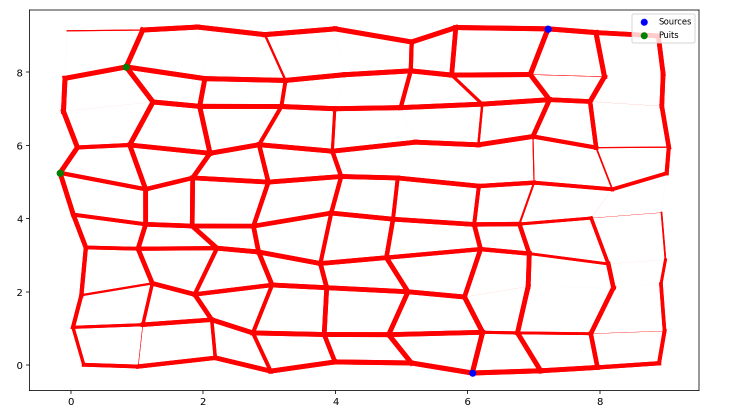
\includegraphics[width=5cm]{blob_debitvar_50.png}
        \caption{$I_{source} = -50 $ et $I_{puit} = 50 $} 
    \end{minipage}
\end{figure}    
\end{center}
\\
Les 3 graphes sont les résultats obtenus après 700 itérations. La première chose que l'on remarque est que plus le débit total (l'intensité) imposé est grand, plus le nombre de branche ayant un flux élevé qui les traverse est grand. Le résultat est le même quand les sources sont immobiles et les puits mobiles ce qui est logique puisque les branches seront aussi larges dans les deux sens de parcours de la nourriture. Nous avons aussi réitérer l'expérience avec des intensités variables sur chaque puits et chaque sources. Il en résulte que les branches seront d'autant plus épaisses ($r$ sera grand) au niveau d'un point que l'intensité, en valeur absolue, sera grande en ce point.
\newpage

\hspace*{1cm}Nous avons développé un maillage triangulaire qui fonctionne selon toutes les règles citées précédemment mais où les polygones formés sont des triangles et chaque point -hormis ceux sur les bords- a six voisins. Nous avons voulu voir ce qu'il se passerait si l'on fixait une source et qu'à chaque pas de temps, la position des puits variait. Voici le résultat pour une source et trois puits avec un maillage triangulaire :

\begin{figure}[h]
    \begin{minipage}[c]{.46\linewidth}
        \centering
        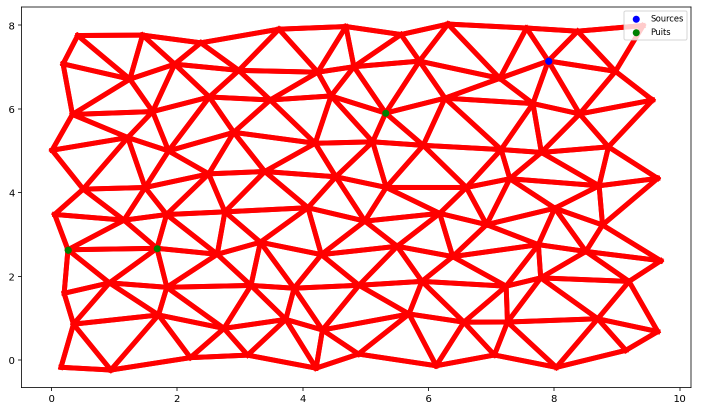
\includegraphics[width=5cm]{Triangle_puit_variable1.png}
        \caption{Blob initial}
    \end{minipage}
    \hfill%
    \begin{minipage}[c]{.46\linewidth}
        \centering
        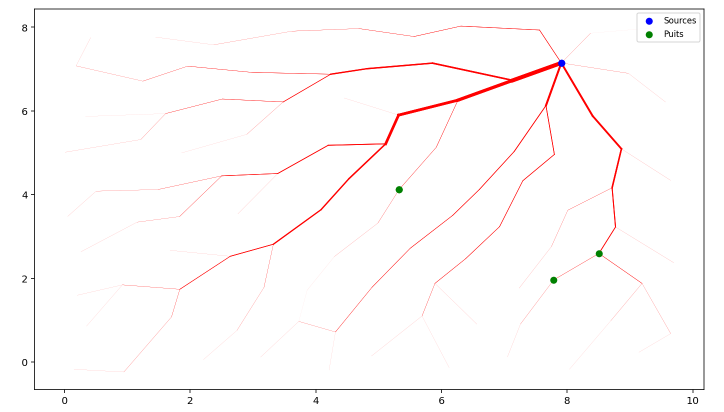
\includegraphics[width=5cm]{Triangle_puit_variable2.png}
        \caption{Blob après 1000 itérations} 
    \end{minipage}
\end{figure}
\FloatBarrier
\end{center}

\hspace*{1cm}Des scientifiques japonais avaient réussi à montrer que le blob était capable de retrouver la structure du réseau du chemin de fer japonais. Nous pouvons voir que notre simulation illustre ce comportement. Imaginons que la source (point bleu) correspond à une grande ville comme Paris. Dans cette analogie, les branches représentent les routes reliant Paris aux villes voisines. Plus une branche est épaisse, plus la route est empruntée par les voyageurs. Autrement dit, plus une branche est épaisse, plus la probabilité qu'un puit s'y trouve à proximité est élevée. Ainsi nous voyons un réseau routier optimisé qui permet de relier Paris aux villes voisines.\\

\hspace*{1cm}On se retrouve avec globalement le même réseau si on fixe les puits et non plus les sources ce qui est logique étant donné que les mêmes chemins se développent, même si les acheminements se font dans le sens inverse, la conductivité ne change pas.

\begin{figure}
    \begin{minipage}[c]{.46\linewidth}
        \centering
        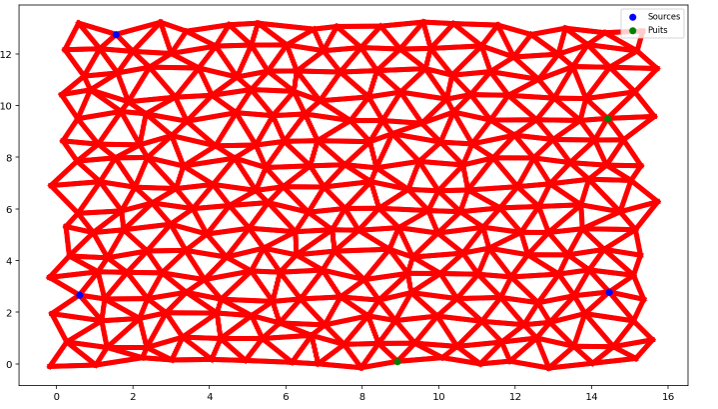
\includegraphics[width=5cm]{source1.png}
        \caption{Blob initial}
    \end{minipage}
    \hfill%
    \begin{minipage}[c]{.46\linewidth}
        \centering
        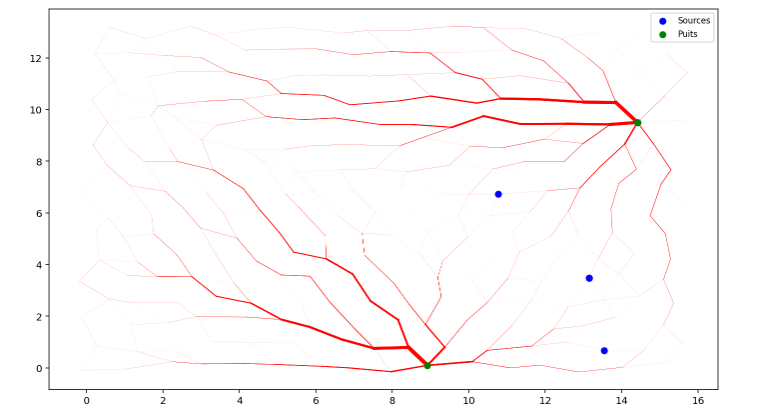
\includegraphics[width=5cm]{source2.png}
        \caption{Blob après 1000 itérations} 
    \end{minipage}
\end{figure}
\FloatBarrier
\end{center}

\hspace*{1cm}Dans la simulation suivante, nous avons fait varier les positions des puits et des sources à chaque pas de temps :

\begin{figure}[h]
    \begin{minipage}[c]{.30\linewidth}
        \centering
        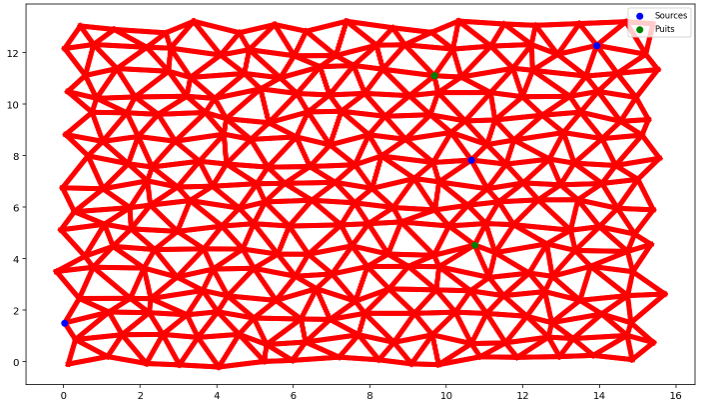
\includegraphics[width=5cm]{puits_sources1.png}
        \caption{Situation initiale}
    \end{minipage}
    \hfill%
    \begin{minipage}[c]{.30\linewidth}
        \centering
        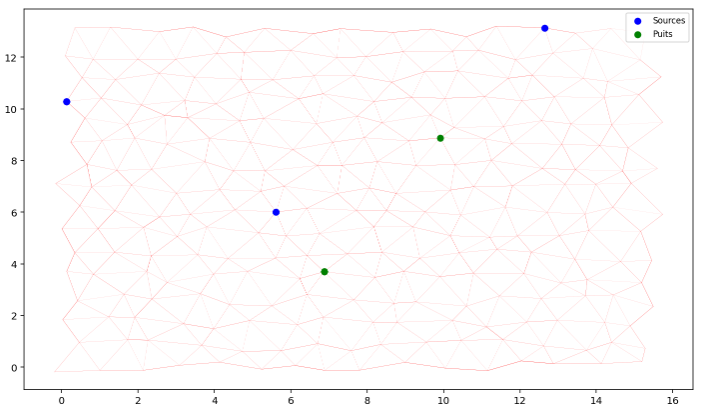
\includegraphics[width=5cm]{puits_sources2.png}
        \caption{Après 500 itérations}
    \end{minipage}
    \hfill%
    \begin{minipage}[c]{.30\linewidth}
        \centering
        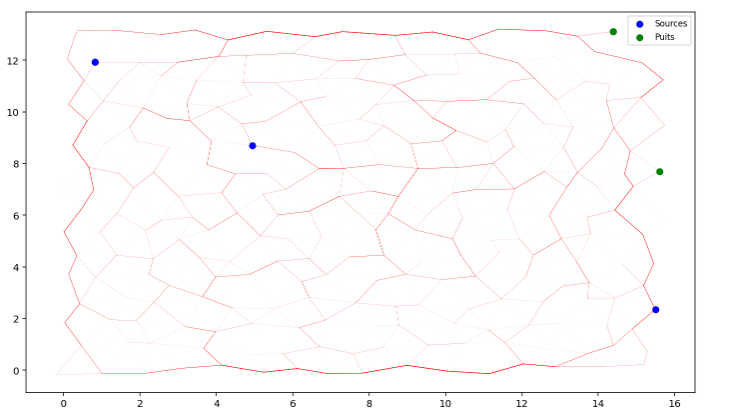
\includegraphics[width=5cm]{puits_sources3.png}
        \caption{Après 1000 itérations} 
    \end{minipage}
\end{figure}
\FloatBarrier
\\
\ \\
\ \\
\\
On observe que dans le cas où les sources et les puits ne sont pas fixes, la conductivité de tous les chemins décroît jusqu'à atteindre un certain stade à partir duquel le blob sélectionne quelles branches il délaisse et lesquelles il garde. Le blob se retrouve donc avec un maillage beaucoup plus espacé et un réseau périphérique s'installe. Étant donné que les puits et les sources sont mobiles, le blob ne garde que les chemins "utiles" permettant de relier facilement deux points alétoirement placés sur les nœuds.
\\
\\
\hspace*{1cm}Nous avons par la suite fait une \href{https://fr.wikipedia.org/wiki/Triangulation_de_Delaunay}{triangulation de Delaunay} à partir d'un nuage de points aléatoire. On utilise \href{https://fr.wikipedia.org/wiki/Marche_de_Jarvis}{la marche de Jarvis} qui permet d'obtenir un polygone convexe qui englobe le nuage de point à partir de points de ce dernier. Ensuite on obtient une triangulation quelconque grâce à \href{https://fr.wikipedia.org/wiki/Triangulation_d%27un_polygone}{la méthode des oreilles} à partir de cette dernière on procède à un \href{https://fr.wikipedia.org/wiki/Triangulation_de_Delaunay#Une_d%C3%A9finition_visuelle_:_le_basculement}{basculement} ce qui permet de transformer deux triangles avec un angle obtus qui forment un quadrilatère, avec donc deux sommets en communs, en deux triangles avec uniquement des angles aigus respectant ainsi les conditions de Delaunay.
\\
\begin{center}
\begin{figure}[h]
    \begin{minipage}[c]{.30\linewidth}
        \centering
        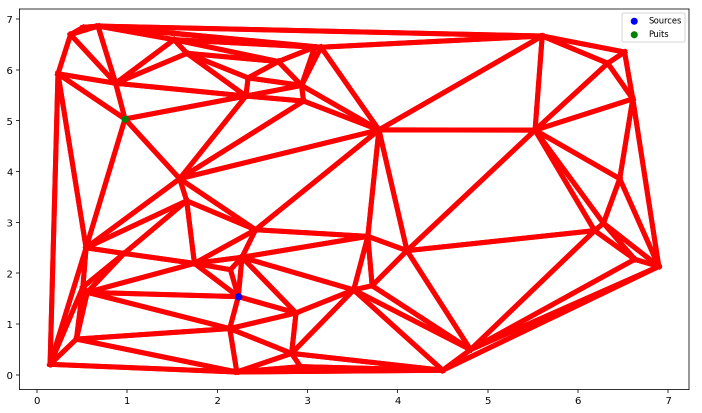
\includegraphics[width=5cm]{delaunay1}
        \caption{Situation initiale}
    \end{minipage}
    \hfill%
    \begin{minipage}[c]{.30\linewidth}
        \centering
        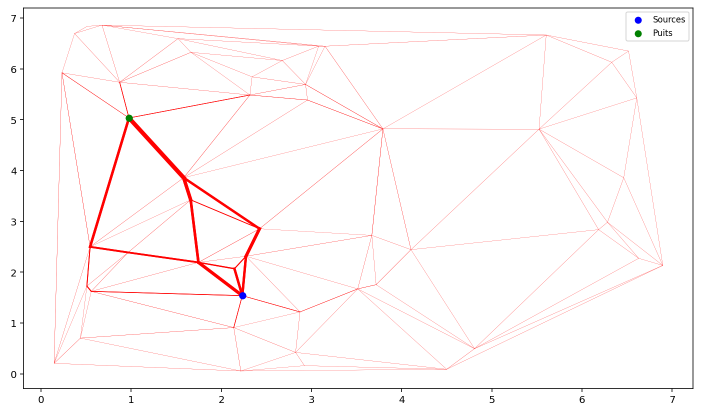
\includegraphics[width=5cm]{delaunay2}
        \caption{Après 500 itérations}
    \end{minipage}
    \hfill%
    \begin{minipage}[c]{.30\linewidth}
        \centering
        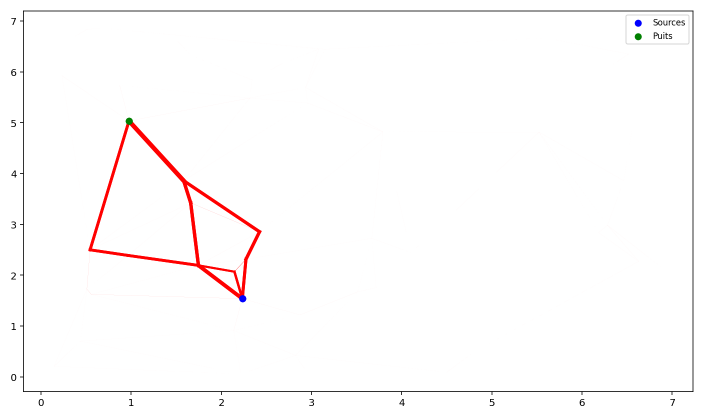
\includegraphics[width=5cm]{delaunay3}
        \caption{Après 1000 itérations}
    \end{minipage}
    \begin{minipage}[c]{.30\linewidth}
        \centering
        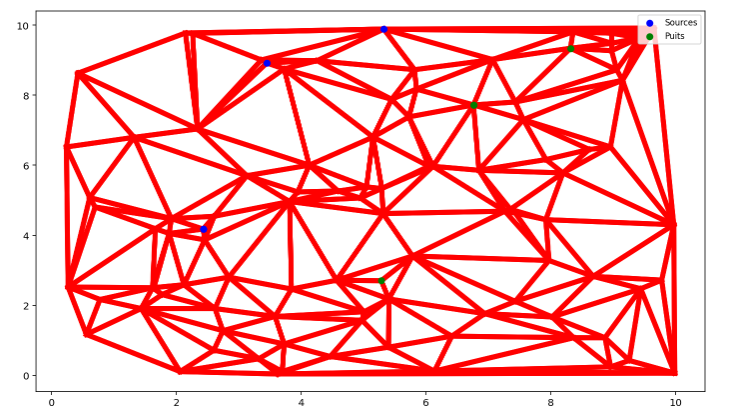
\includegraphics[width=5cm]{delaunay4.png}
        \caption{Situation initiale}
    \end{minipage}
    \hfill%
    \begin{minipage}[c]{.30\linewidth}
        \centering
        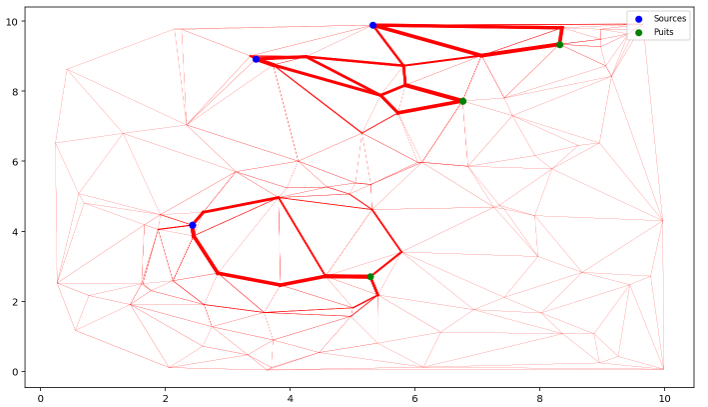
\includegraphics[width=5cm]{delaunay5.png}
        \caption{Après 500 itérations}
    \end{minipage}
    \hfill%
    \begin{minipage}[c]{.30\linewidth}
        \centering
        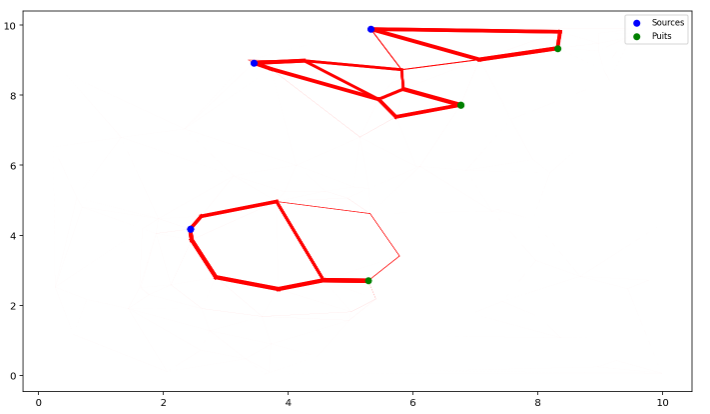
\includegraphics[width=5cm]{delaunay6.png}
        \caption{Après 1000 itérations}
    \end{minipage}
\end{figure}
\end{center}
\FloatBarrier
\hspace*{1cm}Sans grande surprise, le blob a le même comportement que sur un maillage rectangulaire : il cherche à relier les sources et les puits de manière optimale.
\\
\\
\hspace*{1cm} Nous avons essayé avec un autre maillage, en trois dimensions cette fois, que l'on appellera maillage cubique. Ce maillage est relativement différent des autres car on voit bien que pour optimiser ses trajets le blob reste sur la même stratégie qu'avant (à savoir un jeu de branche reliant tous les puits et sources deux à deux de manière optimale). Cependant on observe des branches annexes qui mettent beaucoup plus de temps à s'effacer.

\begin{center}
\begin{figure}[h]
    \begin{minipage}[c]{.30\linewidth}
        \centering
        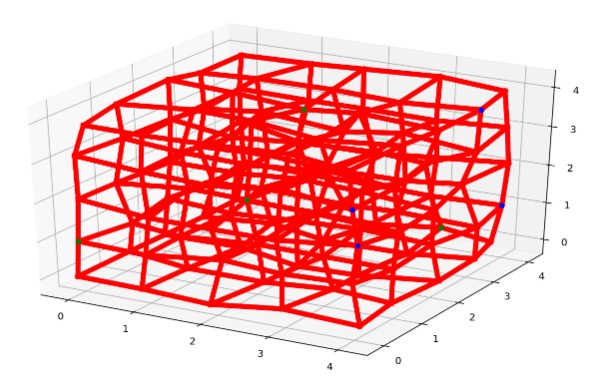
\includegraphics[width=5cm]{blob3D1.png}
        \caption{Situation initiale}
    \end{minipage}
    \hfill%
    \begin{minipage}[c]{.30\linewidth}
        \centering
        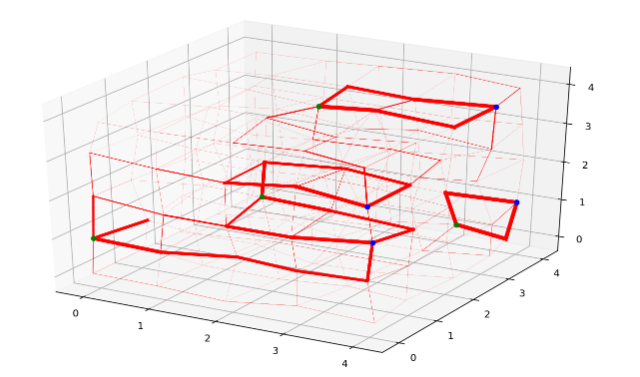
\includegraphics[width=5cm]{blob3D2.png}
        \caption{Après 500 itérations}
    \end{minipage}
    \hfill%
    \begin{minipage}[c]{.30\linewidth}
        \centering
        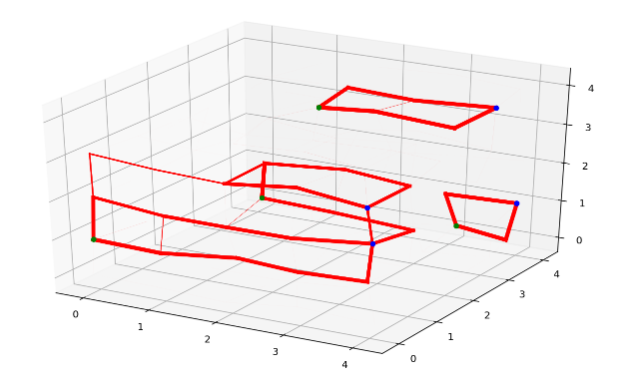
\includegraphics[width=5cm]{blob3D3.png}
        \caption{Après 1000 itérations}
    \end{minipage}
\end{figure}
\end{center}
\FloatBarrier

\section{Éxecution du code}
\hspace*{1cm}Pour faire tourner les simulations, nous avons codé une interface graphique avec le module \textbf{tkinter} de Python. Elle consiste en une liste de boutons correspondant à chaque paramètre de la simulation. La recherche de documentation pour ce module nous ayant posé particulièrement problème.\\

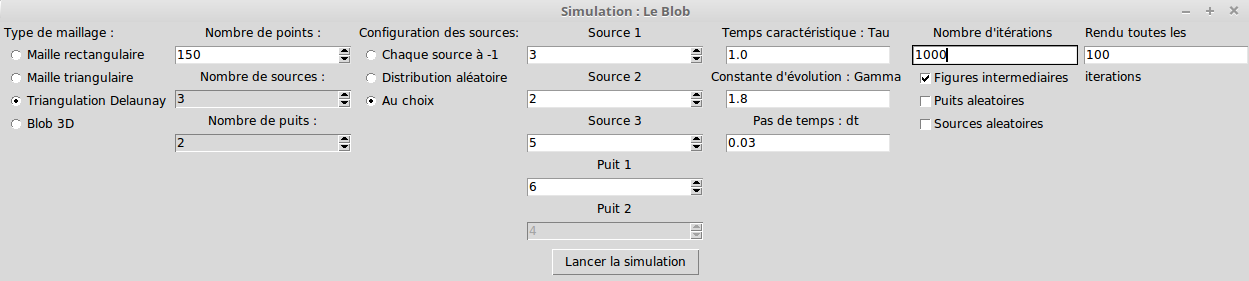
\includegraphics[width=16.5cm]{Interface.png}
        \caption{Situation initiale}
\\
\\
\hspace*{1cm}Malheureusement cette interface ne fonctionne pas si le code est exécuté sur serveur, il faut donc se contenter d'appeler les fonctions avec leur paramètres : la documentation étant fournie dans le fichier .ipynb. Pour ouvrir l'interface il faut donc travailler avec le fichier .py en local.

\section{Conclusion}
\hspace*{1cm}À travers ce projet nous avons pu simuler informatiquement le comportement d'un blob en présence de sources et de puits de nourriture et ainsi nous rendre compte que ce dernier choisissait stratégiquement les branches du maillage à entretenir et celles à délaisser. À travers les nombreux maillages étudiés, nous avons pu constater que le blob arrivait à reproduire ce comportement quelque soit le maillage initial. Cependant lorsque les sources et/ou les puits changeaient de place à chaque pas de temps le blob développait des embranchements en ne gardant actives que les routes "utiles". Les paramètres de l'expérience, $\tau$ et de $\gamma$, n'influent que sur la vitesse de l'expérience et non pas sur le résultat final. Les résultats obtenus montrent cependant que le blob est capable, par exemple, de trouver le moyen de transport optimal entre un nombre donné de point de départ (source) et de point d'arrivée (puit). En matière d'optimisation on pourrait aussi simuler un trafic ferroviaire en modifiant l'intensité des point d'arrivée en fonction de la population d'une ville ce qui permettrait de savoir combien de trains il faudrait envoyer par heure dans certaines gares. Évidemment le blob trouve son utilité dans les problèmes impliquant des réseaux avec des débits que ce soit en hydrostatisque ou en électrocinétique dans des circuits fermés avec des sources de courants et des "puits"/annihilateur de courant. En guise d'ouverture, il serait possible d'étendre le problème du blob à des  dimensions plus élevées ou de travailler avec des sources à l'extérieur du blob et de rajouter la possibilité au blob de déplacer ses nœuds moyennant un coût en énergie.

\newpage

\begin{center}
\title{\Huge\textbf{{Los Commandos}}}
\end{center}

\begin{center}
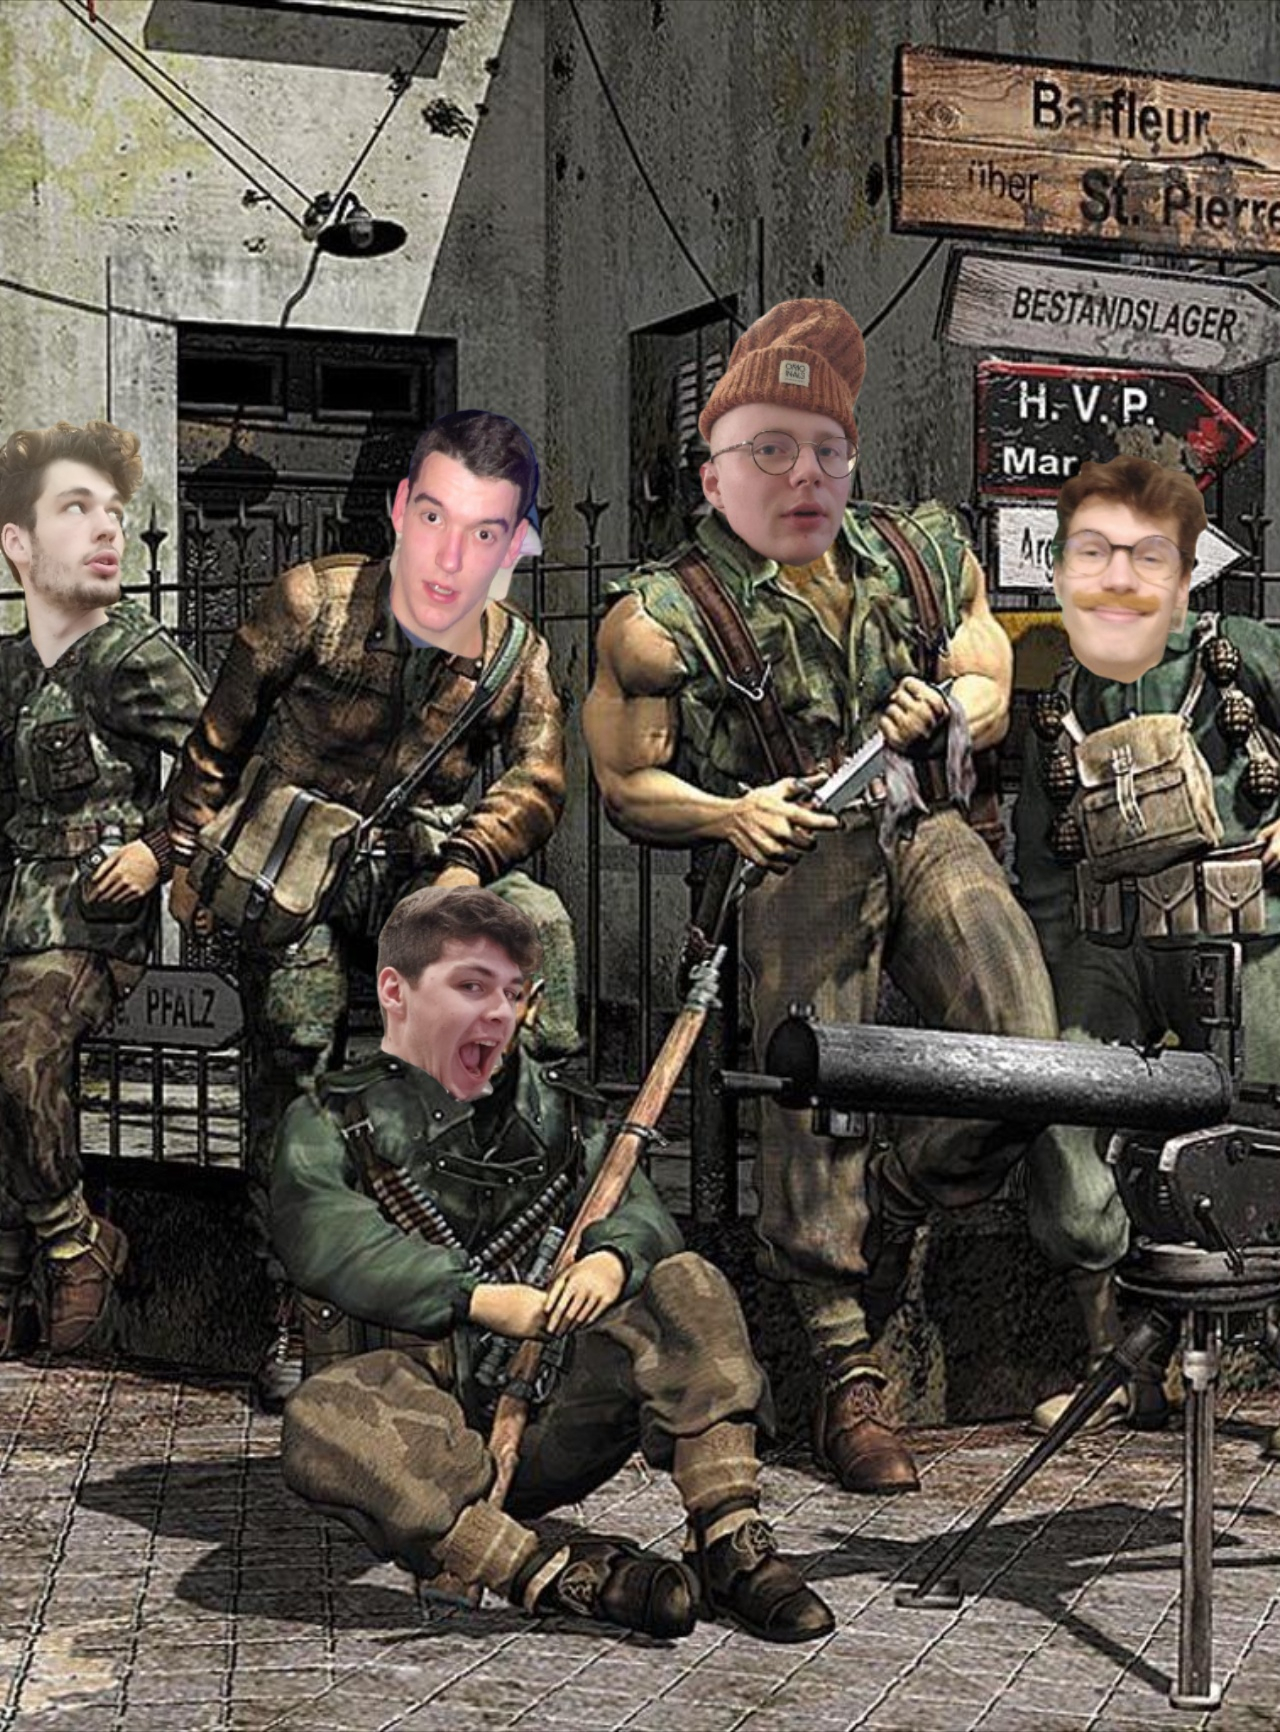
\includegraphics[width=10cm]{Los_commandos.jpg}
\end{center}


\end{document}